%************************************************
\chapter{Developer Guide}\label{ch:developer_guide} % $\mathbb{ZNR}$
%************************************************

This chapter will guide the reader through the different requirements and their implementation in the application.

Having finished with the requirements a section highlighting certain problems or special cases that were encountered during the development will be described.

\section{Implementation of the requirements}
\label{sec:implementation_requirements}

\subsection{Web-requirements}

Requirements \texttt{WR01}, \texttt{WR02} and \texttt{WR03} are implemented in the \texttt{PageHandler}-class:

It requests a provided \ac{URL} via its \texttt{FetchUrl()}-method that will return a \texttt{SimpleWebResponse}-object. The \texttt{SimpleWebResponse}-object encapsulates just a title, body and a url - all elements needed to display a web-page.

To fulfil requirement \texttt{WR04} it is necessary to assign a \texttt{WebResponse} after catching an exception that is thrown by the \texttt{.NET}-framework if a response does not contain a 200 (OK)-message:

\begin{lstlisting}[caption=Fetching \ac{URL}s with error-codes]
try
{
       this.Request = WebRequest.Create(this.RequestUrl);
       this.Response = this.Request.GetResponse();
}
catch (WebException e)
{
       logger.Error("WebException ({0}) occured when fetching the url: {1}", e.Message, this.RequestUrl);
       this.Response = e.Response;
}
\end{lstlisting}

\texttt{WR04} is implemented in the \texttt{PagePresenter}: the page-presenter starts a \texttt{FetchUrl()}-method-call via an asynchronous delegate and provides a callback-mechanism to its \texttt{Done()}-method.

\begin{lstlisting}[caption=Fetching \ac{URL}s with error-codes]
Func<SimpleWebResponse> method = pageHandler.FetchUrl;
method.BeginInvoke(Done, method);
\end{lstlisting}

When the \texttt{Done()}-method is invoked, the presenter calls the view's \texttt{DisplayWebpage()}-method that prints the received \ac{HTML}-code\footnote{See \autoref{subsubsec:view} to see details of the necessary view-implementation.}.

\subsection{Homepage-Requirements}

The homepage is saved as a simple string. This leads to the possibility to save it via the \texttt{ApplicationSettings}\footnote{See \href{MSDN}{http://msdn.microsoft.com/en-us/library/k4s6c3a0.aspx} (\url{http://msdn.microsoft.com/en-us/library/k4s6c3a0.aspx}) for more information} - a facility provided by the \texttt{.NET} framework.

The only problem in this implementation is the fact that only the \texttt{WinForms} project is allowed to access the application-settings\footnote{It would be possible to provide a reference to the \ac{GUI}-project in the logic-project. However this would lead to a dependency between the logic-project and the \ac{GUI} - a circumstance that should be prevented by utilizing the \ac{MVP}-pattern. Due to this fact the \ac{GUI} writes the application settings and the logic stays independent from the \ac{GUI}.}.

Due to this reason the code to write the string is located in the \texttt{SettingsWindow}:

\begin{lstlisting}[caption=Saving the homepage-settings.]
private void SaveSettings(String homePage)
        {
            Settings settings = Settings.Default;
            settings.Homepage = homePage;
            settings.Save();
        }
\end{lstlisting}

\subsection{Favourite-requirements}

The requirements \texttt{FR01} and \texttt{FR02} were implemented in the \texttt{Favourite} and \texttt{FavouriteHandler}-classes.

Apart from handling the adding (\texttt{AddEntry()}), deleting (\texttt{DeleteFavourite()}) and editing (\texttt{EditFavourite()}) of favourites, the \texttt{FavouriteHandler} also handles the saving (\texttt{SaveFavourite()}) and loading (\texttt{LoadFavourites()}) of favourites.

Requirement \texttt{FR04} is fulfilled by the  \texttt{FavouritePresenter}: upon creation, the presenter determines the file-path for the favourite file and sets it in the \texttt{FavouriteHandler}:

\begin{lstlisting}[caption=Setting up the favourite handler's filepath.]
private void SetUpHandler()
        {
            String appFolder = Environment.GetFolderPath(Environment.SpecialFolder.ApplicationData);
            String history = "Favourites.xml";
            this._FavouriteHandler.SetFilePath(Path.Combine(appFolder, history));
            this._FavouriteHandler.LoadFavourite();
        }
\end{lstlisting}

This approach was chosen to keep the \texttt{FavouriteHandler} reusable, whereas the presenter is already closely tied to a concrete implementation, being responsible for handling the information flow.

Requirement \texttt{FR03} was implemented in the \ac{GUI}: when the user clicks an element in the favourite-list, the element is determined and the url of the favourite is written into the \ac{URL}-text-field. After this has happened, a standard \ac{URL}-request is issued and the \ac{URL} will be displayed in the active tab.

\subsection{History-requirements}

The implementation of the history-requirements is similar to the those of the favourites.

The main-classes are \texttt{History} and \texttt{HistoryHandler}, whereas the loading on start-up is provided by the \texttt{HistoryPresenter}.

\begin{lstlisting}[caption=Setting up the history handler's filepath.]
private void SetUpHandler()
        {
            String appFolder = Environment.GetFolderPath(Environment.SpecialFolder.ApplicationData);
            String history = "History.xml";
            this._HistoryHandler.SetFilePath(Path.Combine(appFolder, history));
            this._HistoryHandler.LoadHistory();
        }
\end{lstlisting}

The loading of a \ac{URL} on user-interaction is implemented in the \ac{GUI} via a \texttt{NodeMouseClick-Event} on the \texttt{History-TreeView}.

\subsection{Printing-requirements}

Requirement \texttt{PR01} was implemented in the \texttt{MainWindow} and the \texttt{PrintPresenter}-classes.

The \texttt{PrintPresenter}'s \texttt{Print()}-method will be called for every page that needs to be printed.

The method will determine the size of the String that shall be printed and set the \texttt{HasMorePages}-property to true if the String would not fit onto one page:

\begin{lstlisting}[caption=Printing.]
public void Print(System.Drawing.Printing.PrintPageEventArgs e)
        {
            
            Font font = _PrintView.CurrentFont;
            int charactersOnPage = 0;
            int linesPerPage = 0;

            // Sets the value of charactersOnPage to the number of characters 
            // of PrintString that will fit within the bounds of the page.
            e.Graphics.MeasureString(PrintString, font,
                e.MarginBounds.Size, StringFormat.GenericTypographic,
                out charactersOnPage, out linesPerPage);

            // Draws the string within the bounds of the page
            e.Graphics.DrawString(PrintString, font, Brushes.Black,
                e.MarginBounds, StringFormat.GenericTypographic);

            // Remove the portion of the string that has been printed.
            PrintString = PrintString.Substring(charactersOnPage);

            // Check to see if more pages are to be printed.
            e.HasMorePages = (PrintString.Length > 0);
        }
\end{lstlisting}

\subsection{User-interface requirements}

All actions can be performed via a \ac{GUI}: see \autoref{ch:user_guide} for an introduction of how to use the provided \ac{GUI}.

As the \ac{GUI} was implemented via the \texttt{WinForms} designer and all actions that are not just altering the \ac{GUI} are passed to the presenters, no significant logic that has not already been mentioned is implemented in the \ac{GUI}.

Due to this fact no more implementation-details about the requirements \texttt{GR01} and \texttt{GR02} will be described.

\section{Details of the implementation}
\label{sec:details_implementation}

Apart from just providing an overview over the requirements and their corresponding implementation, this section will provide an overview over certain areas of code that might be hard to understand without further explanation, but are not directly linked to a certain requirement.

\subsection{View}
\label{subsubsec:view}

All \ac{GUI} classes have a common ancestor: the class \texttt{ThreadingView}:

\begin{figure}[H]
\begin{center}
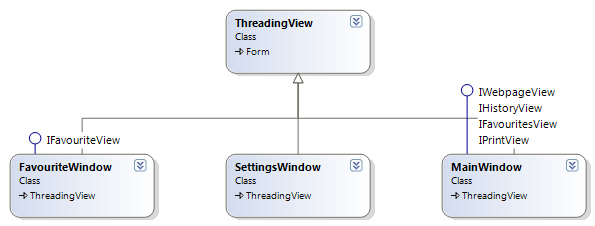
\includegraphics[width=\textwidth]{gfx/view_diagram.png}
\caption{\ac{GUI} class hierarchy}
\label{fig:view_diagram}
\end{center}
\end{figure}

Due to this approach all classes are able to use the \texttt{UpdateUI()}-method of this class when another thread wants to alter a \ac{GUI}-control:

\begin{lstlisting}[caption=Updating the \ac{GUI} from the \ac{GUI}-thread.]
protected void UpdateUI(MethodInvoker uiDelegate)
        {
            if (InvokeRequired)
            {
                this.Invoke(uiDelegate);
            }
            else
            {
                uiDelegate();
            }
        }
\end{lstlisting}

This is necessary as only the thread that created a \ac{GUI}-component is allowed to update it.
Via \texttt{InvokeRequired} it is possible to check if another thread tries to modify the component (returns \texttt{true} if another thread wants to modify it, \texttt{false} otherwise).

In the current application this behaviour might occur when the page-request-thread calls the \texttt{PagePresenter's} \texttt{done()} method and the presenter tries to force the view to display the web-page.
To prevent an exception from ocurring the code to update the \ac{GUI}-component is called like this:

\begin{lstlisting}[caption=Displaying the web-page from the \ac{GUI}-thread.]
public void DisplayWebPage(SimpleWebResponse response)
        {
            foreach (TabPage page in this.webSitesTabControl.TabPages)
            {
                if (page.Name.Equals(response.Url))
                {
                    MethodInvoker uiDelegate = delegate
                    {
                        page.Controls[0].Text = response.Html;
                        page.Text = response.Title;
                    };
                    UpdateUI(uiDelegate);
                }
            }
        }
\end{lstlisting}

This way the \ac{GUI}-thread will alter the component.

\subsection{Observer-pattern}

As already mentioned in \autoref{subsec:separate_change} the observer pattern is used to keep the different presenters up-to-date.
Namely this approach concerns the \texttt{Favourite-} and \texttt{HistoryHandlers} and their respective presenters.

However the implementation was not performed utilizing multiple classes as described in \textcite{gamma1994}, but by utilizing \texttt{.NET} specific concepts like delegates.

Therefore the handlers declare a delegate that the observers can use.
Moreover an event needs to be declared that will chain the multiple methods of the observers, so that every observer will be notified of occuring changes.

The concrete implementation-stubs look like this:

\begin{lstlisting}[caption=Declaration of delegate and event.]
public delegate void ChangeHandler(object subject);
public event ChangeHandler ChangeEvent;
\end{lstlisting}

When a change occurs the \texttt{Notify()}-method will be called that notifies all observers of the change:

\begin{lstlisting}[caption=Notifying observers.]
private void Notify()
{
      if (ChangeEvent != null)
      {
           ChangeEvent(this);
      }
}
\end{lstlisting}

The observers can then handle the change in their subscribed method.

To subscribe, the following chaining to the event is sufficient:

\begin{lstlisting}[caption=Registering as an observer.]
this._HistoryHandler.ChangeEvent += new HistoryHandler.ChangeHandler(this.Update);
\end{lstlisting}

After that the \texttt{Update()}-method can handle all changes:

\begin{lstlisting}[caption=Handling changes in the observer.]
public void Update(object subject)
{
      if (subject is HistoryHandler)
      {
          HistoryHandler histhandler = subject as HistoryHandler;
          this._HistoryView.DisplayHistory(histhandler.History);
      }
}
\end{lstlisting}
% TODO Fancy overview.

\subsection{Singleton-pattern}

Another pattern that was used in the \texttt{Handler}-classes was the \texttt{Singleton}-pattern.

The pattern was employed due to the fact that two different presenters access each handler and both presenter need to modify the same data.

However, the implementation of the singleton is the standard one found in many object-oriented languages:

\begin{lstlisting}[caption=Thread-safe lazy-initialization.]
private static HistoryHandler _Instance;

/// <summary>
/// Gets the instance.
/// </summary>
/// <value>The instance.</value>
public static HistoryHandler Instance
{
            get
            {
                if (_Instance == null)
                {
                    lock (lockObject)
                    {
                        if (_Instance == null)
                        {
                            _Instance = new HistoryHandler();
                        }
                    }
                }
                return _Instance;
            }
        }
\end{lstlisting}

\subsection{Serialisation}
\label{subsubsec:serialisation}

The last thing to be pointed out is the implementation of the persistence-functionality.

The two classes responsible to persist the data (\texttt{FavouriteHandler} and \texttt{HistoryHandler}) refer to the persisting class only via its interface (\texttt{ISerialiser<T>}) making use of polymorphism. This way the implementation can easily be swapped out to support a different kind of serialisation.

In the delivered application the persisting of the history and the favourites is performed via the \ac{XML}-format. Should another format be used it suffices to create a new class that implements the \texttt{ISerialiser<T>}-interface and provide the new mechanism for serialisation.

Then it is enough to instantiate an instance of this new class in the two handlers.

Due to the fact that the current implementation utilises \texttt{Generics} one class can be used for multiple classes.

However, while implementing the application certain limitations of the \texttt{.NET}-framework made it necessary to ``implement"\footnote{The used implementation was taken from \url{http://weblogs.asp.net/pwelter34/archive/2006/05/03/444961.aspx} - as stated in the comments this implementation was tested against 30 test-cases and due to this fact preferred to a self-implemented one.} a new \texttt{SerializableDictionary}-class, as the dictionaries provided by the .NET framework are not serialisable to an \ac{XML}-representation.
